\section*{Problem 6}

In this problem we are asked to find the minimum number of elements needed to 
force the \textit{Non-increasing First Fit Bin-Packing Algorithm} to fit the
items into three bins when the optimum number is two.
\\
\\
We offer the following solution using six elements.

Given the following set of data: $4,4,3,3,3,3$ the algorithm will pack the bins as follows:
\begin{center}
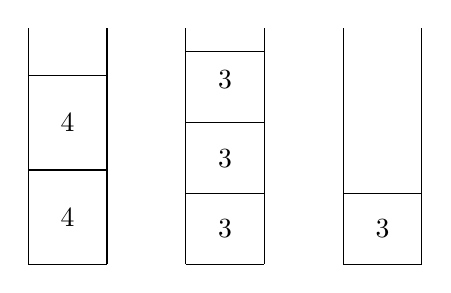
\begin{tikzpicture}
    \draw (0,0) -- (0, -1) -- (0, -2) -- (0, -3)
    (1,0) -- (1, -1) -- (1, -2) -- (1, -3)
    (0, -3) -- (1, -3)
    (0, -1.8) -- (1, -1.8)
    (0, -0.6) -- (1, -0.6);
    
    \node at (0.5,-1.2) {$4$};
    \node at (0.5,-2.4) {$4$};
    
    \draw (2,0) -- (2, -1) -- (2, -2) -- (2, -3)
    (3,0) -- (3, -1) -- (3, -2) -- (3, -3)
    (2, -3) -- (3, -3)
    (2, -2.1) -- (3, -2.1)
    (2, -1.2) -- (3, -1.2)
    (2, -0.3) -- (3, -0.3);
    
    \node at (2.5,-0.65) {$3$};
    \node at (2.5,-1.65) {$3$};
    \node at (2.5,-2.55) {$3$};
    
    \draw (4,0) -- (4, -1) -- (4, -2) -- (4, -3)
    (5,0) -- (5, -1) -- (5, -2) -- (5, -3)
    (4, -3) -- (5, -3)
    (4, -2.1) -- (5, -2.1);
    
    \node at (4.5,-2.55) {$3$};
    
\end{tikzpicture}
\end{center}

Where the optimal backing is 

\begin{center}
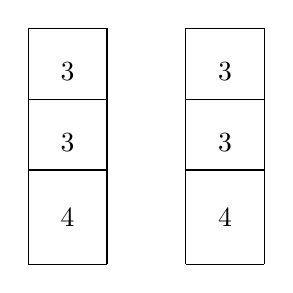
\begin{tikzpicture}
    \draw (0,0) -- (0, -1) -- (0, -2) -- (0, -3)
    (1,0) -- (1, -1) -- (1, -2) -- (1, -3)
    (0, -3) -- (1, -3)
    (0, -1.8) -- (1, -1.8)
    (0, -0.9) -- (1, -0.9)
    (0, -0) -- (1, -0);
    
    \node at (0.5,-0.55) {$3$};
    \node at (0.5,-1.45) {$3$};
    \node at (0.5,-2.4) {$4$};
    
    \draw (2,0) -- (2, -1) -- (2, -2) -- (2, -3)
    (3,0) -- (3, -1) -- (3, -2) -- (3, -3)
    (2, -3) -- (3, -3)
    (2, -1.8) -- (3, -1.8)
    (2, -0.9) -- (3, -0.9)
    (2, -0) -- (3, -0);
    
    \node at (2.5,-0.55) {$3$};
    \node at (2.5,-1.45) {$3$};
    \node at (2.5,-2.4) {$4$};
    
\end{tikzpicture}
\end{center}